\subsection{Experimental results}

To examine selection fairness beyond the theoretical bounds, we conduct simulation-based experiments that reflect Helix's fairness properties in practice. We isolate specific elements within the system and inspect their effect on fairness. We simulate primaries that follow the $b'$-construction strategy and measure fairness as the ratio $b'/b$.    
Our open-source code is available online~\cite{githubconsensus}.
   
To obtain probabilistic results we repeat the same experiment a thousand times and give an average case analysis. In our experiments a pair of nodes, a primary $p$ and a committee member $i$, construct and validate a block respectively. We model their Epools at locking time, $EP_p$ and $EP_i$, by sampling random $etx$s, where the total number of pending $etx$s is $10b$ and $|EP_p \cap EP_i|=\alpha \cdot10b$. The block size is set to $b=1000$.       

\begin{figure}[t!]
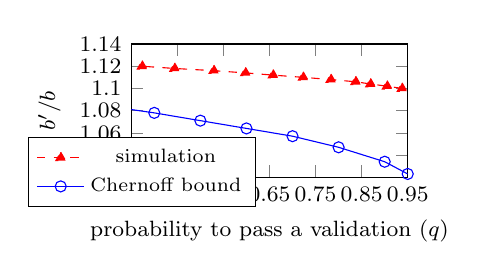
\begin{tikzpicture}
  \begin{axis}
  [ 
    xlabel={probability to pass a validation ($q$)},
    ylabel={$b'/b$},
    xmin=0.35, xmax=0.95,
    ymin=1.02, ymax=1.14,
    xtick={0.35,0.45,0.55,0.65,0.75,0.85,0.95},
    ytick={1.02,1.04,1.06,1.08,1.1,1.12,1.14},
    height = 0.27 \textwidth,
    width = 0.42  \textwidth, 
    legend style={at={(0.45,0.3)},font=\fontsize{7}{5}\selectfont},
    x tick label style={
    	font=\footnotesize,
        /pgf/number format/.cd,
            fixed,
            precision=2,
        /tikz/.cd
    },
    y tick label style={font=\footnotesize},
    label style={font=\footnotesize}
  ] 

       \addplot[color=red, mark=triangle*, dashed] coordinates {(0.9377,1.100)(0.9053,1.102)(0.8693,1.104)(0.8371,1.106)(0.7833,1.108)(0.7231,1.110)(0.6578,1.112)(0.5979,1.114) (0.5292,1.116)(0.4441,1.118) (0.3736,  1.120)
    };
    \addlegendentry{simulation};
    \addplot[color=blue, mark=o] coordinates {
    (0.1,  1.100)(0.2,  1.091)(0.3,  1.084)(0.4,  1.078)
    (0.5,  1.071)(0.6,  1.064)(0.7,  1.057)
    (0.8,  1.047)(0.9,  1.034)(0.95,  1.023)
    };
    \addlegendentry{Chernoff bound}; 
  \end{axis}
\end{tikzpicture}
\caption{The ratio $b'/b$ vs. the desired probability to pass a single validation.}
 \label{fig_pr_vs_q}
\end{figure}

Fig.~\ref{fig_pr_vs_q} illustrates our first experiment. We set $\alpha=0.95$, and check the relation between the primary's desired probability to pass a single validation, $q$, and the maximal $b'$ she can use. We compare the theoretical lower bound to the experimental results. It is interesting to note that the practical results indicate a very moderate decent from $q=0.95$ to $q=0.5$ where $b'$ increases by roughly $20$ $etx$s. This should imply that rational primaries would use $b'<1100$ (and avoid unnecessary risks). Note that within these (less than) $100$ extra $etx$s there is only a fraction of promoted ones, see Fig.~\ref{fig_tx_inclusion_prob}. In case we take larger $b$s or $\alpha$s the relative amount of feasible manipulation further reduces.

In a real system, the Chernoff bound could serve as ``advice" to the primary, as to what $b'$ she can use and still pass validation with her desired probability. An upper bound analysis, that would indicate the maximal $b'$ a primary might use and still pass a single validation with a desired probability, is left for future work.

\begin{figure}[t!]
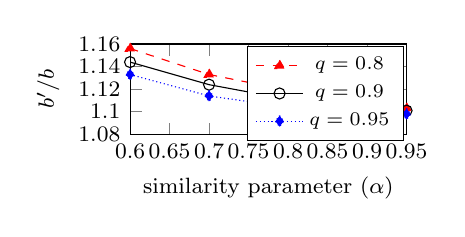
\begin{tikzpicture}
  \begin{axis}[ 
    xlabel= similarity parameter ($\alpha$),
    ylabel={$b'/b$},
    xmin=0.60, xmax=0.95,
    ymin=1.08, ymax=1.16,
    xtick={0.60,0.65,0.70,0.75,0.80,0.85,0.90,0.95},
    ytick={1.08,1.10,1.12,1.14,1.16},
        height = 0.2250 \textwidth,
    width = 0.42  \textwidth, 
    legend style={at={(0.990,0.980)},font=\fontsize{7}{5}\selectfont},
    x tick label style={
    	font=\footnotesize,
        /pgf/number format/.cd,
            fixed,
            precision=2,
        /tikz/.cd
    },
    y tick label style={font=\footnotesize},
    label style={font=\footnotesize}
  ] 
 % \addplot {(1-x*1.12) / (1-x)};
   % \addplot gnuplot [domain=0.1:0.5,samples = 10 ]{(1-x*1.12) / (1-x) }; 
     \addplot[color=red, mark=triangle*, dashed] coordinates {
(0.6, 1.156)
(0.7, 1.133) 
(0.8, 1.119)
 (0.85, 1.111)
 (0.9, 1.107) 
(0.95, 1.103)
    };
    \addlegendentry{$q=0.8$}; 
       \addplot[color=black, mark=o] coordinates {
(0.6, 1.144) 
(0.7, 1.124) 
(0.8, 1.111) 
(0.85, 1.105) 
(0.9, 1.102)
(0.95, 1.101)
    };
    \addlegendentry{$q=0.9$}; 
          \addplot[color=blue, mark=diamond*,densely dotted] coordinates {
(0.6, 1.133) 
(0.7, 1.114) 
(0.8, 1.104) 
(0.85, 1.101) 
(0.9, 1.098)
(0.95, 1.098)
    };
    \addlegendentry{$q=0.95$}; 
  \end{axis}
\end{tikzpicture}
\caption{Impact of network similarity parameter on fairness---larger $\alpha$ values enhance fairness.}
 \label{fig_ratio_vs_alpha}
\end{figure}

Fig.~\ref{fig_ratio_vs_alpha} illustrates the second experiment which checks the effect of $\alpha$ on selection fairness. It clearly shows that larger $\alpha$ yields smaller $b'/b$ ratio. Intuitively, large $\alpha$ values allow the validator to know more about the primary's Epool thus yielding stricter validation conditions (i.e., larger $\beta$), resulting in enhanced fairness. %The value of $\alpha$ is affected by various network characteristics .  

Finally, Fig.~\ref{fig_tx_inclusion_prob} takes into account the analysis in Lemma~\ref{Fairness_WRT_Pormoted_Lemma} and the fraction of $etx$s the primary wishes to promote in order to give a realistic estimation of the possible manipulation in $b'$-constructions. We choose $b'$ values arising from the simulations presented in Fig.~\ref{fig_pr_vs_q}. For non-promoted $etx$s, the graph shows the ratio between the probability of getting included in $b'$-constructions, to that in the $b$-construction. We plot these ratios with respect to different fractions of $etx$s, $\xi_p$, the primary wishes to promote. 
The fact that the observed ratios are very close to $1$ (even for small $q$ values) demonstrates that in practice, selection fairness in \name is maintained even under a $b'>b$ manipulation.

\begin{figure}[t!]
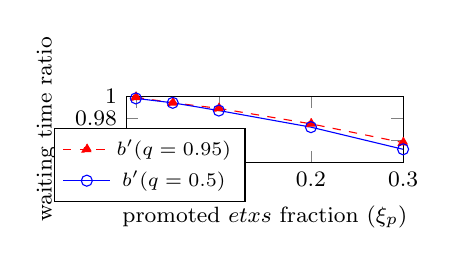
\begin{tikzpicture}
  \begin{axis}[ 
    xlabel= promoted $etxs$ fraction ($\xi_p$),
    ylabel={waiting time ratio},
 %   ylabel={fairness ratio},
    xmin=0, xmax=0.3,
    ymin=0.94, ymax=1,
    xtick={0.01,0.1,0.2,0.3},
    ytick={0.94,0.96,0.98,1},
        height = 0.200 \textwidth,
    width = 0.42  \textwidth, 
    legend style={at={(0.43,0.525)},font=\fontsize{7}{5}\selectfont},
    x tick label style={
    	font=\footnotesize,
        /pgf/number format/.cd,
            fixed,
            precision=2,
        /tikz/.cd
    },
    y tick label style={font=\footnotesize},
    label style={font=\footnotesize}
  ] 
 % \addplot {(1-x*1.12) / (1-x)};
   % \addplot gnuplot [domain=0.1:0.5,samples = 10 ]{(1-x*1.12) / (1-x) }; 
     \addplot[color=red, mark=triangle*, dashed] coordinates {
       (0.01 ,0.999 )
(0.05 ,0.994 )
(0.1 ,0.989 )
(0.2 ,0.975 )
(0.3 ,0.958 )
    };
    \addlegendentry{$b'(q=0.95)$}; 
       \addplot[color=blue, mark=o] coordinates {
 (0.01 ,0.998 )
(0.05 ,0.994 )
(0.1 ,0.987 )
(0.2 ,0.972 )
(0.3 ,0.952 )
    };
    \addlegendentry{$b'(q=0.5)$}; 
  \end{axis}
\end{tikzpicture}
\caption{The ratio between the expected waiting time of a non-promoted $etx$ in the $b$-construction, and that in a $b'$-construction. In both curves $\alpha=0.95$.
}
 \label{fig_tx_inclusion_prob}
\end{figure}

However, the main insight from the experiment section is that, surprisingly, the effectiveness of the selection fairness scheme is quite indifferent to the similarity parameter $\alpha$. Between $\alpha=0.95$ and $\alpha=0.6$, the ratio $b'/b$ and the expected waiting time of non-promoted $etx$s does not differ by much. Thus, in practice, a system that uses our selection fairness mechanism should not make a special effort to increase $\alpha$. 

We note however that in the experiments above, the parameter $\alpha$ used for validation matched the actual overlap of Epools. We believe that a loose estimation of $\alpha$ would enable primaries to manipulate \nameNS's selection fairness, e.g., by tailoring many $etx$s. It is left for future work to find methods to reduce the importance of estimating $\alpha$ accurately.   


